\documentclass[11pt]{article}
\usepackage[margin=1in]{geometry}
\usepackage[T1]{fontenc}
\usepackage{lmodern}
\usepackage{microtype}
\usepackage{graphicx}
\usepackage{booktabs}
\usepackage{enumitem}
\usepackage[hidelinks]{hyperref}
\setlist{nosep, leftmargin=1.5em}

\title{Formal Verification for Coding-Agent Memory Rules}
\author{CS2520 Project Report}
\date{December 2026}

\begin{document}
\maketitle

% ---------------------------------------------------------------------------
\section{Introduction}

Coding agents such as Claude Code keep project rules in memory files (\texttt{CLAUDE.md},
\texttt{.claude/memory/}) that load into every session~\cite{claudecode-memory}. Users and agents
add rules over time, sometimes within a single session. A new rule is appended as text, and
nothing checks it against the rules already there. Two problems follow. Rules can clash, so that
no action follows all of them. And agents can break rules that are loaded: in our trial, Claude
Code broke a memory rule in 8 of 30 runs with the rule files present.

Today the agent is the only reader of its memory rules: it sees them in its prompt and decides on
its own whether to follow them. To our knowledge, no separate step checks a new rule for clashes
when it is written, or checks an action against the rules before it runs. We study two ways to add
such a step: a language model that reads the rules in English, and the Z3
solver~\cite{z3}. Z3 gives the same answer every time and checks in milliseconds, but only for
rules written in logic. This leads to our question: \emph{is formal verification useful for agent
memory, and where?}

We borrow the policy-as-code idea (Open Policy Agent~\cite{opa}, AWS Cedar~\cite{cedar}). A
language model translates each rule once into constraints over a fixed schema of git commands,
file actions, tasks and a few yes/no facts; output that names anything outside the schema, or does
not compile, is rejected. Z3 then checks the rules at two points:
\begin{itemize}
  \item \textbf{Memory update:} does a new rule clash with the rules already there?
  \item \textbf{Agent action:} does the step the agent is about to take break a rule? If so, block it.
\end{itemize}
The schema guarantees a checkable form, but not that the translation means the same as the English
rule.

The results split along one line: whether a rule fits the schema. On all real action rules (334
actions), the language models beat Z3, with F1 0.87 (DeepSeek) and 0.85 (Haiku) against 0.78;
every Z3 miss is a rule it cannot express or a translation gap. On rules Z3 can express (101
actions), Z3 wins, 0.97 against 0.90 and 0.89. For clashes, a language model reading the whole
folder found more: only 5 of 22 labelled clashes fit Z3's logic. In live agent runs, the Z3 gate
flagged 8 of 8 runs with a break, blocked 4 of 4 attempted breaks, and raised no false flags.

Our contributions are:
\begin{itemize}
  \item a schema-constrained translation of memory rules into Z3, with a clash check and an action gate;
  \item studies comparing Z3 with language-model judges, on public memory folders and in live agent runs;
  \item \texttt{memclash}, an extension for the Pi coding agent~\cite{pi} that applies both checks to a live agent.
\end{itemize}

Our results support a narrow claim. For rules that fit the schema, a Z3 gate is cheap and fast,
and adding a rule costs one translation, not a re-read of the whole memory. Agents follow their
memory rules in most runs; the breaks we saw are edge cases, such as reading \texttt{.env} while
debugging, but those edge cases are what a gate is for. Rules outside the schema remain open:
future work is to bring more of them into a checkable form, or to find other cheap ways to check
them when a rule is added.

% ---------------------------------------------------------------------------
\section{Method}

Figure~\ref{fig:pipeline} shows the final pipeline. We first describe the approaches that led to
it, then each step.

\subsection{What we tried first}

\paragraph{One format for every rule.} Our first design translated every memory rule into one
general record, borrowing from access control (the subject, resource, action and conditions of
XACML~\cite{xacml} and attribute-based access control~\cite{abac}) and from deontic logic (whether an
action is required, forbidden or permitted~\cite{vonwright}). Words for actions and scopes came
from an open list, linked by hand-written relations such as ``\texttt{pip} excludes \texttt{uv}''.
Checked by Z3, this design found 0 of 10 labelled conflicts. Tools that check rules exactly work on
subjects whose vocabulary is fixed in advance; ours was open.

\paragraph{A fixed model, first for git only.} We therefore narrowed the exact method to rules
about git, over a fixed list of operations (commit, push, merge, \ldots) and facts about them
(branch, user asked, tests passed). Cedar~\cite{cedar}, AWS's policy language, is built for
access decisions: each policy permits or forbids a single request at the moment it is made. Memory
rules are different in kind: they also require actions and order them across a session (``run the
linter before you commit''), and our clashes arise between such rules. We therefore kept Cedar's
approach, a fixed vocabulary checked by a solver, but not its language. A survey of further memory folders showed that rules about files
and about running commands are as common as git rules and can be written in the same fixed form,
so the vocabulary was extended to the schema in Section~\ref{sec:schema}.

\paragraph{Keeping what cannot be expressed.} Our first translations dropped conditions the
schema has no words for, so ``never commit in the local clones'' became ``never commit'' and
clashed with every rule that requires a commit. On the large folders all 20 reported clashes were
false. Dropping a condition widens a rule and creates false clashes, so conditions are now kept as
unknown facts (Section~\ref{sec:translate}); the false clashes went to 0.

\subsection{Schema}\label{sec:schema}

\paragraph{Where it comes from.} The schema combines two sources. The first is existing
policy-as-code and permission systems: GitHub rulesets~\cite{gh-rulesets}, Claude Code
permissions~\cite{cc-permissions}, Cedar~\cite{cedar} and AppArmor~\cite{apparmor}. All of them fix
the list of actions in code and leave only names (branches, paths, commands) open; we follow the
same design, so the schema changes only through a new version, never during translation. The
second is the memory folders we collected: 200 public memory folders from GitHub, gathered in
three batches. The first 100 showed which actions rules are about. Besides git, these are file
actions (read, create, edit, move, delete) and running commands such as tests and builds; these
became the action list, and rules about tool choice, writing style or plan steps were left outside.
The clause types follow deontic logic~\cite{vonwright}: \texttt{never} (prohibition),
\texttt{must\_do} (obligation), \texttt{may\_do} (permission) and \texttt{only\_if} (an action
allowed only under a condition). The schema was drafted with two AI reviewers over several rounds
and approved by the author.

\paragraph{Structure.}
A rule is translated into clauses about one agent action. Each clause has a type and a
\emph{where} part that says which actions it covers, and some types have a \emph{needs} part
(Appendix~\ref{app:schema}, Table~\ref{tab:schema}). The vocabulary is fixed in code; any other name is an error.

For example, ``Never read any \texttt{.env} file, except \texttt{.env.example}'' becomes
\texttt{never \{cmd: read, path: [.env, .env.*], path\_except: [.env.example]\}}, and ``Only push a
branch after its tests have passed'' becomes \texttt{only\_if \{cmd: push\} needs \{tests\_passed\}}.
Each clause compiles into quantifier-free Z3 constraints over a symbolic action, with paths and
branch names as Z3 strings matched by regular expressions.

\subsection{Translation and schema check}\label{sec:translate}

An LLM (DeepSeek 4.1 Flash) translates one rule at a time and sees only the rule, its file name
and its section heading, never the other rules, so that other rules cannot change how a rule is
read. We compared two ways to translate. In \emph{one step}, the model reads the rule and writes
all its clauses in a single answer. In \emph{two steps}, the model first splits the rule into
single requirements, each with the exact words it comes from and the words that limit when it
applies; in a second call it translates each requirement into clauses, or leaves it out as vague,
outside the vocabulary, or using an unclear word. On our development set, two steps gave fewer
malformed answers and more correctly classified rules, so it became the default. A likely reason
is that a long rule often hides several requirements, and listing them first keeps the model from
dropping one.

Every answer is checked against a JSON schema and the vocabulary, and must compile to Z3. A
failing answer is sent back once with the error; if it fails again the rule is marked invalid and
counted, never guessed. A condition the schema cannot express (``in the local clones'') is kept as
an unknown yes/no fact, so the clause applies only when that fact holds. The check guarantees a
checkable form, not that the translation means what the English rule means.

\subsection{Clash check}

Two rules clash if, in some situation the rules name, no single action satisfies both. Z3 searches
for such a situation and action. ``May'' is read as a strong permission: the action must stay
possible, so ``you may skip the tests for doc-only changes'' clashes with ``always run the tests''
and is reported as an \emph{exception} that needs a priority rule. A clash that holds only when an
unknown fact is true is reported as a \emph{possible clash}. In scoring, every verdict (clash,
exception, state conflict, possible clash) counts as a flag: it is correct if the pair really
conflicts and a false alarm otherwise, with no partial credit. When every pair is compatible, a
group check asks whether all rules can still be followed together, since some clashes need three
rules.

\subsection{Action gate}

Before the agent acts, its tool call is mapped to schema events: a shell command becomes, for
example, a branch switch, a commit and a push, with the current branch and the session's earlier
steps (which tests ran, and whether they passed). For each event, Z3 checks every \texttt{never}
and \texttt{only\_if} clause; if one is broken, the action is blocked and the agent is shown the
rule's own text. Clauses that depend on an unknown fact are switched off, so the gate blocks only
what it can check. \texttt{must\_do} and \texttt{may\_do} clauses cannot be broken by a single
action and are left to the clash check.

\begin{figure}[t]
  \centering
  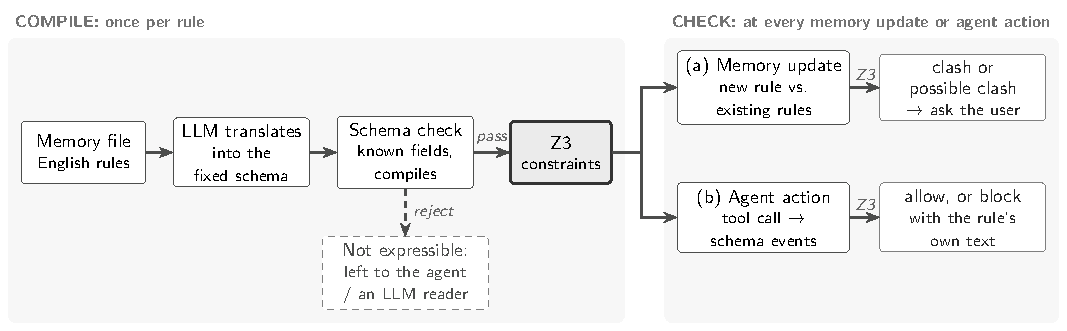
\includegraphics[width=\textwidth]{fig1_pipeline.pdf}
  \caption{Pipeline. Each English rule is translated once into constraints over a fixed schema;
  output that fails the schema check is rejected and left to the agent or an LLM reader. Z3 then
  checks at two points: (a) when a rule is added, against the existing rules, and (b) before each
  agent action, against all rules.}
  \label{fig:pipeline}
\end{figure}

% ---------------------------------------------------------------------------
\section{Studies and Results}\label{sec:results}

\subsection{Set-up}

We test the two checks of Section~2 in four studies, each planned before its runs. Rules come from
the public memory folders of Section~\ref{sec:schema}. Actions and clash pairs were labelled by two
AI labellers, with disagreements settled by the author. The baselines are two LLM judges, DeepSeek
4.1 Flash and Claude Haiku 5.5, which read the same rules in English and decide directly, without
translation. We report F1 for catching rule breaks, so that missed breaks and wrongly blocked
actions both count.

\subsection{Stopping rule breaks}

On all real action rules (334 actions), the LLM judges catch more rule breaks than Z3: F1 0.87 for
DeepSeek and 0.85 for Haiku, against 0.78 (Appendix~\ref{app:results}, Table~\ref{tab:f1}). Z3
rarely blocks an allowed action, so its loss comes from missed breaks. Every miss falls on a rule
the schema cannot express, or on one translated only in part. A partial translation still keeps
the rule's core action, which most breaking actions hit, which is why Z3 still catches most
breaks.

When the test is limited to rules the schema can express (101 actions), Z3 scores higher than both
judges: 0.97, against 0.90 and 0.89. Its few misses came from translation, not from the solver.

Across both sets, the solver decided every translation correctly; every Z3 error traces back to
translation, whether a rule outside the schema, a condition left out or a wrong field. This matches
the design in Section~\ref{sec:translate}: the schema guarantees a checkable form, not the right
meaning, so translation quality sets Z3's accuracy.

\subsection{Finding clashes}

Clashes are real but mostly fall outside Z3's logic. Across the memory folders of 56 repositories,
12 had at least one clash, 42 in all. Of the 22 clashes labelled in detail, only 5 fit the schema;
most concern which tool or command to use (12 of 22), plan steps, file layout or setting values.
On the pairs with saved translations, Z3 found 1 of 2 clear clashes with one false alarm, while one
LLM call reading the whole folder found both with none. As with the gate, Z3's errors were in
translation: a dropped ``may'', a target with no file path, and a lost scope.

\subsection{Live agent runs}

To test the gate beside a real agent, Claude Code (Sonnet 5.5) ran five tasks in sandboxed
repositories, 10 runs per condition, with the rules visible in \texttt{CLAUDE.md}, only in a topic
file, or buried among 159--394 other rules; two more conditions ran the Z3 gate live.

The agent followed its rules in most runs: 22 of 30 ungated runs had no break, and every break fell
in 2 of the 5 tasks, reading \texttt{.env} while fixing a configuration bug and running tests the
user had not asked for. The gate flagged all 8 runs with a break, with no false flags. Live, it
blocked 4 of 4 attempted breaks, and after each block the agent complied and told the user why.

\subsection{Cost}

Z3 is faster and cheaper at both checkpoints (Appendix~\ref{app:results}, Table~\ref{tab:cost}).
As a gate, Z3 checks an action in about 5\,ms at no cost. An LLM judge needs one call per action,
about 1.5--3\,s and \$0.0002--0.0004, and the cost grows with the number of rules it must read.
Adding a rule takes Z3 about 14\,s and \$0.001, because only the new rule is translated, while
DeepSeek re-reading every rule takes about 3 minutes and \$0.02. Z3's one-time cost is translating
every rule once, about 1 minute and \$0.04. Z3 also gives the same answer on every run.

% ---------------------------------------------------------------------------
\section{Artifact: memclash for Pi}
% TODO

% ---------------------------------------------------------------------------
\section{Limitations}
% TODO

% ---------------------------------------------------------------------------
\section{Conclusion}
% TODO

\bibliographystyle{plain}
\bibliography{refs}

\appendix
\section{Schema}\label{app:schema}

\begin{table}[h!]
  \centering\small
  \begin{tabular}{@{}ll@{}}
    \toprule
    Part & Values \\
    \midrule
    Actions & 18 git operations (commit, push, force push, merge, branch delete, \ldots); \\
            & file read, create, edit, move, delete; \texttt{run} a task (test, build, lint, deploy, \ldots) \\
    Targets & file paths and branch names, with wildcards (\texttt{*} within one folder, \texttt{**} any depth) \\
    Yes/no facts & user asked, user confirmed, tests passed, has a secret, \ldots \\
    Earlier steps & an action that must have happened before, with its branch, task and outcome \\
    Clause types & \texttt{never}, \texttt{only\_if} (needs), \texttt{must\_do}, \texttt{may\_do}, and two state types \\
    \bottomrule
  \end{tabular}
  \caption{The fixed schema (vocabulary v2), summarised from \texttt{pipeline/rules/vocab.py}.}
  \label{tab:schema}
\end{table}

\section{Results}\label{app:results}

\begin{table}[h!]
  \centering\small
  \caption{F1~$\uparrow$ for catching rule breaks. \emph{All rules}: every eligible rule.
  \emph{Expressible}: only rules whose translation two reviewers judged exact.}
  \label{tab:f1}
  \begin{tabular}{@{}lcc@{}}
    \toprule
    & All rules (334 actions) & Expressible (101 actions) \\
    \midrule
    Z3 & 0.78 & \textbf{0.97} \\
    DeepSeek 4.1 Flash & \textbf{0.87} & 0.90 \\
    Claude Haiku 5.5 & 0.85 & 0.89 \\
    \bottomrule
  \end{tabular}
\end{table}

\begin{table}[h!]
  \centering\small
  \caption{Time and cost~$\downarrow$ on a 51-rule memory. Values marked $\sim$ are estimates from
  measured token counts, output speed and API prices.}
  \label{tab:cost}
  \begin{tabular}{@{}lrr@{}}
    \toprule
    & Time & Cost \\
    \midrule
    \multicolumn{3}{@{}l}{\emph{Gate, per action}} \\
    \quad Z3 & \textbf{$\sim$5\,ms} & \textbf{\$0} \\
    \quad Claude Haiku 5.5 & $\sim$1.5\,s & $\sim$\$0.0002 \\
    \quad DeepSeek 4.1 Flash & $\sim$3\,s & $\sim$\$0.0004 \\
    \midrule
    \multicolumn{3}{@{}l}{\emph{Adding one rule}} \\
    \quad Z3 (translate 1 rule, check all) & \textbf{$\sim$14\,s} & \textbf{$\sim$\$0.001} \\
    \quad DeepSeek 4.1 Flash (re-read every rule) & $\sim$3\,min & $\sim$\$0.02 \\
    \bottomrule
  \end{tabular}
\end{table}
\end{document}
